
\documentclass[letterpaper, reqno,11pt]{article}
\usepackage[margin=1.0in]{geometry}
\usepackage{color,latexsym,amsmath,amssymb}
\usepackage{fancyhdr}
\usepackage{amsthm}
\usepackage{mathtools}
\usepackage{tikz}
\usepackage{float}
\usepackage{centernot}
\usepackage{subcaption}
\usepackage{extarrows}
\usetikzlibrary{hobby}
\usetikzlibrary{shapes.multipart}
\usepackage{pgfplots}
\pgfplotsset{compat=1.7}
\usetikzlibrary{arrows.meta}
\usepackage{cancel}
\usetikzlibrary{decorations.markings}
\usetikzlibrary{shapes}
\usetikzlibrary{arrows}
\usepgfplotslibrary{fillbetween}
\usetikzlibrary{patterns}

\newcommand{\RR}{\mathbb{R}}
\newcommand{\CC}{\mathbb{C}}
\newcommand{\ZZ}{\mathbb{Z}}
\newcommand{\QQ}{\mathbb{Q}}
\newcommand{\NN}{\mathbb{N}}
\DeclareMathOperator{\id}{id}
\def\upint{\mathchoice%
  {\mkern13mu\overline{\vphantom{\intop}\mkern7mu}\mkern-20mu}%
  {\mkern7mu\overline{\vphantom{\intop}\mkern7mu}\mkern-14mu}%
  {\mkern7mu\overline{\vphantom{\intop}\mkern7mu}\mkern-14mu}%
  {\mkern7mu\overline{\vphantom{\intop}\mkern7mu}\mkern-14mu}%
  \int}
\def\lowint{\mkern3mu\underline{\vphantom{\intop}\mkern7mu}\mkern-10mu\int}
\DeclareMathOperator{\card}{card}
\DeclareMathOperator{\Binomial}{Binomial}
\DeclareMathOperator{\Span}{span}
\DeclareMathOperator{\sgn}{sgn}
\pagestyle{fancy}
\lhead{Math 321 Lecture 32}
\rhead{Yuchong Pan}
\begin{document}
\pagenumbering{arabic}
\title{Math 321 Lecture 32}
\author{Yuchong Pan}
\date{March 27, 2019}
\newtheorem{thm}{Theorem}
\newtheorem{defn}{Definition}
\newtheorem*{remark}{Remark}
\newtheorem{claim}{Claim}
\newtheorem{cor}{Corollary}
\newtheorem{lemma}{Lemma}
\newtheorem{prop}{Proposition}
\newtheorem{fact}{Fact}
\newtheorem{observation}{Observation}
\maketitle
%

\section{Implicit Function Theorem}

\noindent {\bf Examples:}
\begin{itemize}
\item $x^2 + y^2 + 1 = 0$: no solution $(x, y) \in \RR^2$.
\item $x^2 + y^2 = 0$: exactly one solution $(0, 0)$; no solution of the form $y = g(x), x \in \text{interval}$.
\item $x^2 + y^2 - 1 = 0$.
  Then,
  \begin{align}
    2x + 2y \frac{dy}{dx} &= 0, \nonumber \\
    \Aboxed{\frac{dy}{dx} &= -\frac{x}{y}.} \label{eq:*} \tag{*}
  \end{align}

  \noindent {\bf Case 1 (Good):} $(a, b) = \left(\frac{1}{\sqrt 2}, \frac{1}{\sqrt 2}\right)$. Then we can solve \eqref{eq:*}: $y = \sqrt{1 - x^2}$.

  $(a, b) = \left(-\frac{1}{2}, -\frac{\sqrt 3}{2}\right)$: $y = -\sqrt{1 - x^2}$.

  $\frac{dy}{dx}$ well-defined.

  \begin{figure}[H]
    \centering
    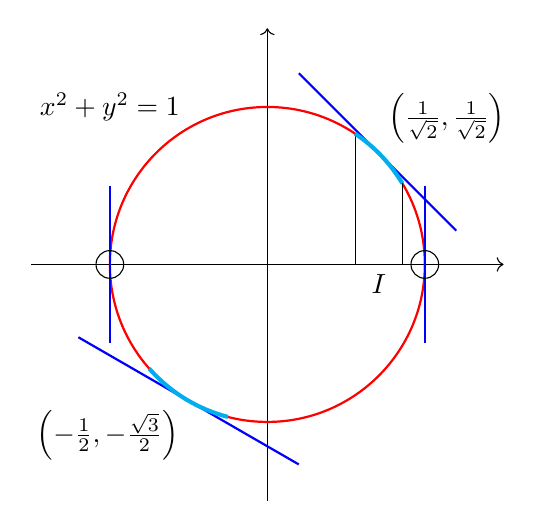
\begin{tikzpicture}
      \draw[->] (-3, 0) -- (3, 0);
      \draw[->] (0, -3) -- (0, 3);
      \draw[red, thick] (0, 0) circle (2);
      \node at (-2, 2) {$x^2 + y^2 = 1$};
      \draw[scale=2, domain=0.2:1.2, variable=\x, blue, thick] plot ({\x},{1.414 - \x});
      \draw[scale=2, domain=-1.2:0.2, variable=\x, blue, thick] plot ({\x}, {-2/3.*sqrt(3) - 0.577*\x});
      \node[above right] at (1.414, 1.414) {$\left(\frac{1}{\sqrt 2}, \frac{1}{\sqrt 2}\right)$};
      \node[below left] at (-1, -1.732) {$\left(-\frac{1}{2}, -\frac{\sqrt 3}{2}\right)$};
      \draw (1.114, 0) -- (1.114, 1.661);
      \draw (1.714, 0) -- (1.714, 1.031);
      \draw[scale=1, domain=1.114:1.714, variable=\x, line width=1.5pt, smooth, cyan] plot ({\x}, {sqrt(4 - \x*\x)});
      \node[below] at (1.414, 0) {$I$};
      \draw[scale=1, domain=-1.5:-0.5, variable=\x, line width=1.5pt, smooth, cyan] plot ({\x}, {-sqrt(4 - \x*\x)});
      \draw[thick, blue] (2, -1) -- (2, 1);
      \draw[thick, blue] (-2, -1) -- (-2, 1);
      \draw (2, 0) circle (5pt);
      \draw (-2, 0) circle (5pt);
    \end{tikzpicture}
  \end{figure}

  \noindent {\bf Case 2 (Bad):} $(a,b) = (1, 0) \text{ or } (-1, 0)$. Solutions to $x^2 + y^2 = 1$ are \emph{not} unique in any neighbourhood of these points; $y = \pm \sqrt{1 - x^2}$ are both possible.

  $\frac{dy}{dx}$ is not meaningful.
\end{itemize}

\begin{thm}[Implicit function theorem]
  \normalfont Let $E \overset{\text{open}}{\subseteq} \RR^{n + m}, n, m \geq 1$ and $\mathbf f : E \to \RR^n, \mathbf f \in C^1(E)$. Suppose $(\underbrace{\mathbf a}_{\in \RR^n}, \underbrace{\mathbf b}_{\in \RR^m}) \in E$ such that $\mathbf f(\mathbf a, \mathbf b) = \mathbf 0$.

  Set $\mathbf A = \mathbf f'(\mathbf a, \mathbf b)_{n \times (n + m)}$. Write $\mathbf A = \left[
    \begin{tabular}{c|c}
      $\underbrace{\mathbf A_x}_{n \times n}$ & $\underbrace{\mathbf A_y}_{n \times m}$
    \end{tabular}
    \right]_{n \times (n + m)}$. Assume $\mathbf A_x$ is invertible.

  \begin{figure}[H]
    \centering
    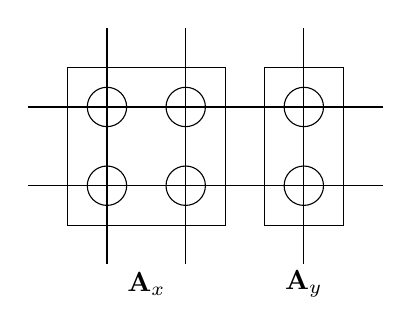
\begin{tikzpicture}
      \draw (0, 0) circle (0.25);
      \draw (1, 0) circle (0.25);
      \draw (0, -1) circle (0.25);
      \draw (1, -1) circle (0.25);
      \draw (2.5, 0) circle (0.25);
      \draw (2.5, -1) circle (0.25);
      \draw (-0.5, 0.5) rectangle (1.5, -1.5);
      \draw (2, 0.5) rectangle (3, -1.5);
      \draw (-1, 0) -- (3.5, 0);
      \draw (-1, -1) -- (3.5, -1);
      \draw (0, 1) -- (0, -2);
      \draw (1, 1) -- (1, -2);
      \draw (2.5, 1) -- (2.5, -2);
      \node at (0.5, -2.25) {$\mathbf A_x$};
      \node at (2.5, -2.25) {$\mathbf A_y$};
    \end{tikzpicture}
  \end{figure}

  \noindent {\bf Conclusion:} There exist open sets $\boxed{U \subseteq E \subseteq \RR^{n + m}}$ and $W \subseteq \RR^m$, $(\mathbf a, \mathbf b) \in U$ such that
  \begin{enumerate}
  \item For every $\mathbf y \in W$, there exists a unique $(\mathbf x, \mathbf y) \in U$ which satisfies the equation $\mathbf f(\mathbf x, \mathbf y) = \mathbf 0$. Define this $\mathbf x$ as $\mathbf g(\mathbf y)$.
  \item $\mathbf g : \underbrace{W}_{\subseteq \RR^m} \to \RR^n$ with $\mathbf y \mapsto \mathbf x$. Then $\mathbf g \in C^1$, with
    \[ \mathbf g'(\mathbf b) = \underbrace{-(\overbrace{\mathbf A_x}^{n \times n})^{-1} \overbrace{\mathbf A_y}^{n \times m}}_\text{$n \times m$ matrix}. \]
  \end{enumerate}
\end{thm}

\begin{proof}
  \renewcommand{\qedsymbol}{}
  
  {\bf Strategy:} Define an auxiliary function $\mathbf F : E \subseteq \RR^{n + m} \to \RR^{n + m}$ on which the inverse function theorem can be applied:
  \[ \mathbf F(\mathbf x, \mathbf y) = (\underbrace{\mathbf f(\mathbf x, \mathbf y)}_{\in \RR^n}, \underbrace{\mathbf y}_{\in \RR^m}), \quad \mathbf x \in \RR^n, \quad \mathbf y \in \RR^m, \quad (\mathbf x, \mathbf y) \in E \subseteq \RR^{n + m}. \]
  Need to verify the hypothesis of the inverse function theorem, namely:
  \begin{itemize}
  \item $\underbrace{\mathbf F}_{= (\mathbf f(\mathbf x, \mathbf y), \mathbf y)} \in C^1(E)$ because each entry is $C^1$;
  \item $\mathbf F'(\mathbf a, \mathbf b)$ is invertible:
    \[ \mathbf F'(\mathbf a, \mathbf b) = \left[
      \begin{tabular}{c|c}
        \multicolumn{2}{c}{$\mathbf A = \mathbf f'(\mathbf a, \mathbf b)_{n \times (n + m)}$} \\
        \hline
        $\mathbf 0_{m \times n}$ & $\mathbf I_{m \times m}$
      \end{tabular}
      \right] = \underbrace{\left[
    \begin{tabular}{c|c}
      $(\mathbf A_x)_{n \times n}$ & $(\mathbf A_y)_{n \times m}$ \\
      \hline
      $\mathbf 0_{m \times n}$ & $\mathbf I_{m \times m}$
    \end{tabular}
    \right]}_{(n + m) \times (n + m)} = \mathbf X. \]

    Note that
    \[ \mathbf X
    \begin{pmatrix}
      \mathbf u \\
      \mathbf v
    \end{pmatrix}
    = \mathbf 0 \quad \Leftrightarrow \quad
    \begin{array}{lcl}
      \mathbf u &=& \mathbf 0 \\
      \mathbf v &=& \mathbf 0
    \end{array}, \]
    because
    \begin{gather*}
      \mathbf A_x \mathbf u + \mathbf A_y \mathbf v = \mathbf 0 \quad \Rightarrow \quad \mathbf A_x \mathbf u = \mathbf 0 \quad \Rightarrow \quad \mathbf A_x^{-1} \mathbf A_x \mathbf u = \mathbf 0 \quad \text{i.e.} \quad \mathbf u = \mathbf 0, \\
      \mathbf 0 \mathbf u + \mathbf I \mathbf v = \mathbf 0 \quad \text{i.e.} \quad \mathbf v = \mathbf 0.
    \end{gather*}
  \end{itemize}

  (Proof unfinished.)
\end{proof}

\end{document}
